\section{Analysis}
\unskip\label{elcc:sec:analysis}

In this section we give present a brief set of analyses that demonstrate some of the possible insights that can be gained from ELCC\@.
% \Cref{tab:quant-sum} shows the five-number summary of the corpus-level metrics in ELCC (full results in \Cref{elcc:sec:big-tables}).
\Cref{tab:quant-sum} shows the five-number summary of the corpus-level metrics in ELCC.
The corpora come in all shapes and sizes, so to speak, demonstrating a wide range of token counts, vocabulary sizes, entropies, and so on.
The variety, in large part, comes from the diversity of systems included in ELCC rather than variation within a system.
Thus research focusing on a single or narrow range of emergent communication systems---the norm prior to ELCC---restricts itself to a limited diversity of corpus ``shapes''; ELCC, in turn, provides an easy opportunity to expand the breadth of many such approaches.

\begin{table}
  \centering
  \inputelcc{src/figure/summary}
  \medskip
  \caption{Five-number summary of the analyses across corpora of \theLib{}.  Entropy in bits.}
  \unskip\label{tab:quant-sum}
\end{table}

The range of analyses ELCC enables is greatly multiplied by a resource like XferBench \citep{xferbench}, a deep transfer learning-based evaluation metric for emergent languages.
This metric quantifies how good a corpus is as pretraining data for a human language-based downstream task, specifically language modelling (thus a lower score is better).
XferBench proves to be particularly powerful for analyzing ELCC because it works in an environment-agnostic way, taking only a corpus of tokenized utterances as input.
In fact, ELCC and XferBench permit the first large-scale comparison of emergent language systems with an \emph{evaluative} metric.


\paragraph{Explaining XferBench's performance}

\begin{figure}
  \centering
  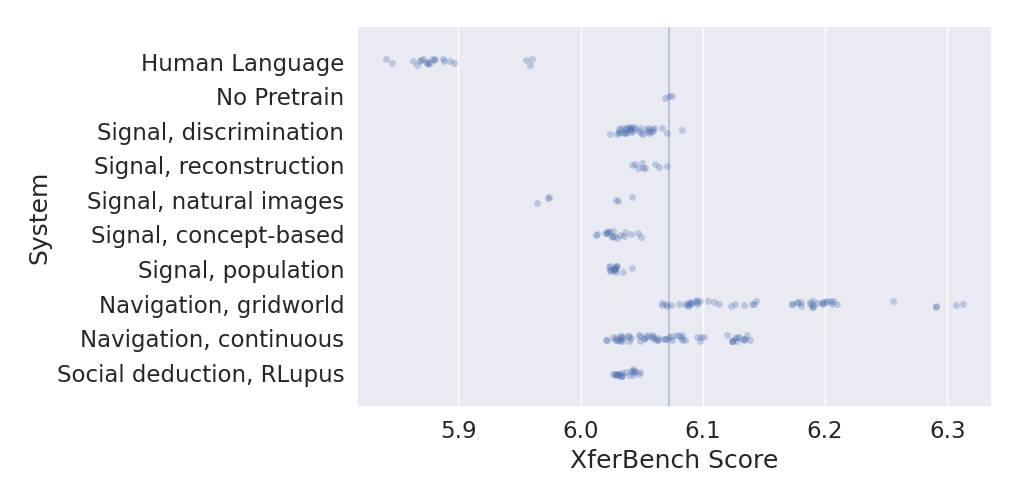
\includegraphics[width=0.7\linewidth]{chapters/elcc/src/figure/generated/elcc-cat}
  \caption{XferBench score across ELCC and human language baselines; lower is better.  ``No pretrain'' baseline illustrated with the line on the plot.}
  \unskip\label{elcc:fig:elcc-cat}
\end{figure}

In addition to the purely descriptive metrics discussed above, we also present evaluative metrics via XferBench in \Cref{elcc:fig:elcc-cat}.
We run XferBench three times for each corpus since there inherent stochasticity in XferBench.
% Compared to the baseline of ``no pretraining'', we see that many of the emergent languages beat this 
We see that most of the emergent languages occupy a band which slightly outperforms the baselines (i.e., no pretraining at all) while significantly underperforming human languages (exception discussed below).
Notably, two of the environments with the worst-performing corpora
  are the grid-world \citep{unger2020GeneralizingEC} and continuous \citep{boldt2023mathmodel} navigation environments, while the signalling games perform better consistently.

\begin{figure}
  \newcommand\hang{\hangindent=0.2in}
  \centering
  \hfill
  \begin{subfigure}{0.45\linewidth}
    \centering
    \fbox{\begin{minipage}{0.9\linewidth}
      \ttfamily\fontsize{8pt}{8pt}\selectfont
      \hang {[47, 2466, 47, 3923, 3325, 3107, 3350, 3923, 1216, 3980, 1617, 3350, 1897, 556, 0]}\par
      \hang {[3925, 3925, 3925, 3325, 1172, 2530, 3925, 1209, 3493, 665, 512, 3923, 2432, 309, 0]}\par
      \hang {[2128, 2128, 2371, 3925, 946, 512, 1962, 1288, 2250, 1722, 1722, 1962, 3755, 2695, 0]}
    \end{minipage}}
    \caption{Best-performing: signalling game \citep{yao2022linking} with the COCO dataset.}
  \end{subfigure}
  \hfill
  \begin{subfigure}{0.45\linewidth}
    \centering
    \fbox{\begin{minipage}{0.9\linewidth}
      \ttfamily\fontsize{8pt}{8pt}\selectfont
      \hang {[3, 3, 3, 3, 3, 3, 3, 3, 7, 7, 7, 7, 7, 7, 7, 7]}\par
      \hang {[3, 3, 3, 3, 3, 3, 3, 3, 3, 3, 3, 3, 3, 3, 3, 3]}\par
      \hang {[3, 3, 3, 3, 3, 3, 3, 3]}
    \end{minipage}}
    \bigskip
    \caption{Worst-performing: BabyAI-based navigation game \citep{unger2020GeneralizingEC} (hyperparameters in text).}
  \end{subfigure}
  \hfill
  \caption{Sample utterances from the best and worst performing emergent language corpora on XferBench from ELCC.}
  \unskip\label{elcc:fig:quale}
\end{figure}

Inspecting some utterances from the best- and worst- performing corpora, we can see a qualitative difference in \Cref{elcc:fig:quale}.
The best-performing corpus uses a variety of tokens derived from a large vocabulary (given the high token IDs), while the worst-performing corpus repeats the same two tokens with little variation (this sample is representative of the whole corpus).
We hypothesize that pretraining on repetitive strings of a small variety of tokens poorly conditions the model used in XferBench, supported by the fact that the lowest entropy corpora perform the worst on XferBench.

\begin{figure}
  \centering
  \hfill
  \begin{subfigure}{0.45\linewidth}
    \centering
    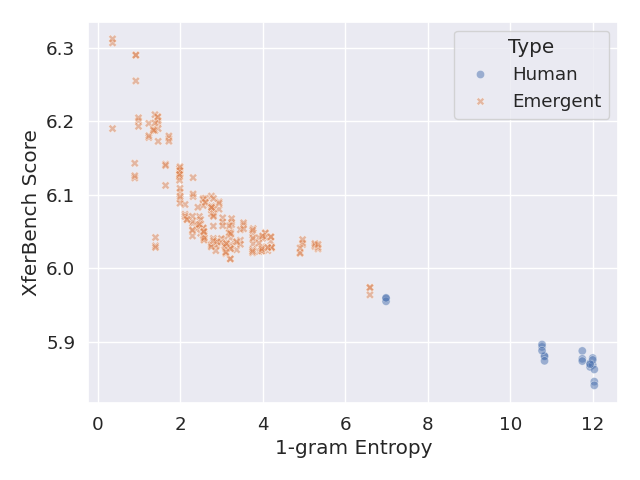
\includegraphics[width=\linewidth]{chapters/elcc/src/figure/generated/entropy-scatter}
    \caption{Plot of XferBench score versus unigram entropy for emergent languages and baseline human languages from XferBench.}
  \end{subfigure}
  \hfill
  \begin{subfigure}{0.45\linewidth}
    \centering
    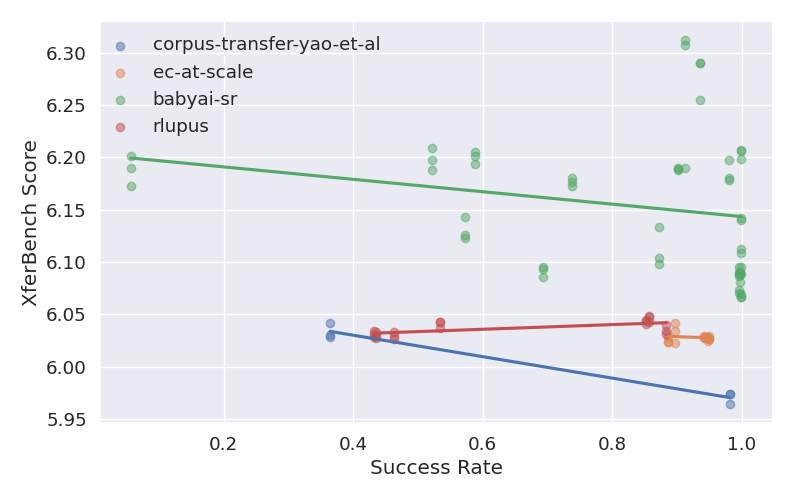
\includegraphics[width=\linewidth]{chapters/elcc/src/figure/generated/success-scatter}
    \caption{Plot of XferBench score versus success rate, separated by emergent communication system.}
  \end{subfigure}
  \hfill
  \caption{}
  \label{elcc:fig:scatter}
\end{figure}

The qualitative analysis suggests that something along the lines of variation or information content might be correlated with XferBench score.
To investigate this, we plot two possible explanatory variables against XferBench scores: unigram entropy and task success rate \Cref{elcc:fig:scatter}.
Immediately, we can see that there is a strong correlation between entropy and XferBench score.
In fact, this plot gives some insight into the anomalously low score on ``Signal, natural images'' \citep{yao2022linking} and anomalously high score for Hindi (an unresolved quandary of the XferBench paper): both of these corpora perform as expected given their entropies.
On the other hand, success rate does not seem to be well-correlated with score on XferBench; surprisingly enough, the worst-performing corpus shown above still sported a ${>}90\%$ task success rate!


\paragraph{Evaluating improvements in ECS design}
\begin{figure}
  \centering
  \hfill
  \begin{subfigure}{0.45\linewidth}
    \centering
    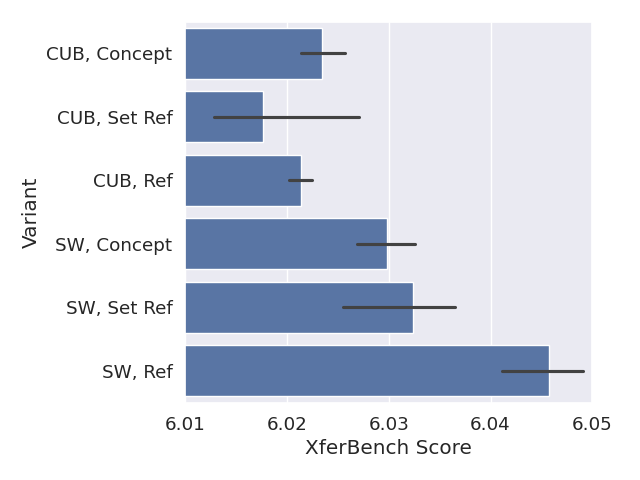
\includegraphics[width=\linewidth]{chapters/elcc/src/figure/generated/mu-goodman}
    \caption{Expected order: concept, set reference, reference \citep{mu2021generalizations}.}
  \end{subfigure}
  \hfill
  \begin{subfigure}{0.45\linewidth}
    \centering
    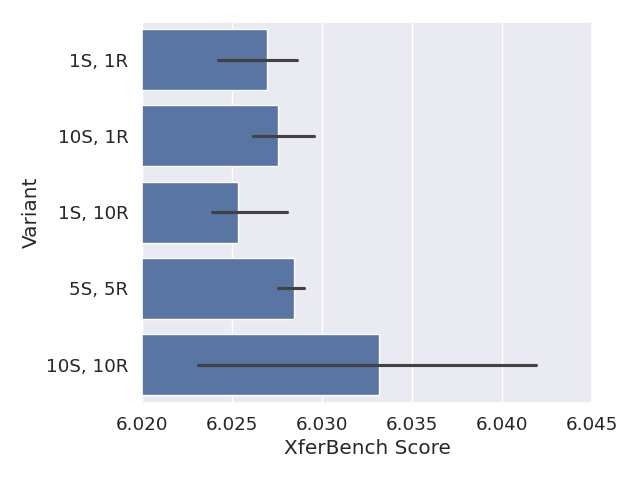
\includegraphics[width=\linewidth]{chapters/elcc/src/figure/generated/ec-at-scale}
    \caption{\# of senders, \# of receivers; more agents expected to perform better than fewer \citep{chaabouni2022emergent}.}
  \end{subfigure}
  \hfill
  \caption{XferBench scores compared to expected order; lower is better.}
  \label{elcc:fig:improvements}
\end{figure}
Finally, we are also able to use XferBench and ELCC to evaluate some of the innovations in emergent communication system design made by papers contributing to ELCC\@.
Namely, we look at \citet{mu2021generalizations} and ``Emergent Communication at Scale'' \citep{chaabouni2022emergent}.
\citet{mu2021generalizations} introduce (as discussed in \Cref{elcc:sec:signalling}) a more sophisticated, concept-focused version of the signalling game, comparing it against a vanilla signalling game (``reference'') and an intermediate form of the concept version (``set reference''), finding that the introduced games promote more systematic and interpretable emergent languages.
On the other hand, \citet{chaabouni2022emergent} introduces multi-agent populations to the signalling game but does not find that larger populations have a beneficial effect on communication.
Looking at the systems' performance XferBench (\Cref{elcc:fig:improvements}), we can see that the proposed improvements to the signalling game do not have an appreciable effect on XferBench performance in either case.
These results do not detract from the original findings; instead, evaluating the design changes with XferBench better contextualizes work, highlighting to what degree certain desirable features of emergent languages (e.g., interpretability, robustness) correspond with suitability for deep transfer learning.

% a\paragraph{Theoretical models}
% a\phantom{}
% a\cmt{nav-to-center experiments and mathematically modelling}
% a\cmt{To include or not?}
